%%% This CHAR topic includes Replication, which is often used as a mean to
%%% implement High Availability. This talk is about the other cases when you
%%% need replication, and will explore interesting compromises that we
%%% sometimes need to make in our implementations.

\documentclass{beamer}

\usepackage{minted}
%% \usemintedstyle{emacs}
\usepackage{beamerthemesplit}
\usepackage[utf8]{inputenc}
%% \usetheme{AnnArbor}
\usetheme{Boadilla}
%% \usetheme{Pittsburgh}
%% \usecolortheme{beaver}
\beamertemplatetransparentcovered

\title{Advanced Distributed Architectures}
\author{Dimitri Fontaine \url{dimitri@2ndQuadrant.fr}}
\date{July 11, 2013}
\logo{
\includegraphics[height=0.4cm]{2ndQuadrant-cross.png}}

\begin{document}

\frame{\titlepage}

\section{Introduction}

\begin{frame}[fragile]
  \frametitle{Dimitri Fontaine}

  \begin{center}
    \textbf{2ndQuadrant France}
    \linebreak
    PostgreSQL Major Contributor
  \end{center}
  \vfill

\begin{columns}[c]
\column{.75\textwidth} 

  \begin{itemize}
   \item<1-> \texttt{pgloader}, \texttt{prefix}, \texttt{skytools}, …
   \item<1-> \texttt{apt.postgresql.org}
   \item<2-> \texttt{\textbf{CREATE EXTENSION}}
   \item<2-> \texttt{\textbf{CREATE EVENT TRIGGER}}
   \item<3-> MySQL migration tool, new \texttt{pgloader} version
  \end{itemize}  

\column{.25\textwidth}
\begin{center}
  
\includegraphics[height=7em]{event-trigger.jpg}
  %% 
\includegraphics[height=5em]{dim-sketch.png}
\end{center}
\end{columns}
\end{frame}

\begin{frame}
  \frametitle{Glossary}
  
  \center{Some vocabulary}
  \vfill

\begin{columns}[c]
\column{.75\textwidth} 

  \begin{itemize}
    \item \alert{C}lustering
    \item \alert{H}igh-\alert{A}vailability \only<2->{\textit{of services or of data?}}
    \item \alert{R}eplication
  \end{itemize}  

\column{.25\textwidth}

\includegraphics[height=6em]{glossaire.jpg}
\end{columns}
\end{frame}

\begin{frame}
  \frametitle{Distributed Architecture, aka\textit{CLUSTER}}

\begin{columns}[c]
\column{.15\textwidth} 
\column{.85\textwidth} 
  
\includegraphics[height=19em]{distribution.jpg}
\end{columns}
\end{frame}

\begin{frame}
  \frametitle{Glossary}
  
  \center{Some vocabulary, \textit{cont.}}
  \vfill

\begin{columns}[c]
\column{.5\textwidth} 

  \begin{itemize}
    \item Architectures
    \item \textit{Distributed Architectures}
    \item Shared Data
    \item Data Shards
    \item Load Balancing
    \item Write Scalability
  \end{itemize}  

\column{.5\textwidth}

\includegraphics[height=12em]{distribution.jpg}
\end{columns}
\end{frame}

\begin{frame}
  \frametitle{Architectures}

  \center{Software Architecture is about how to achieve \textbf{goals}}

\begin{columns}[c]
\column{.1\textwidth} 
\column{.9\textwidth} 
  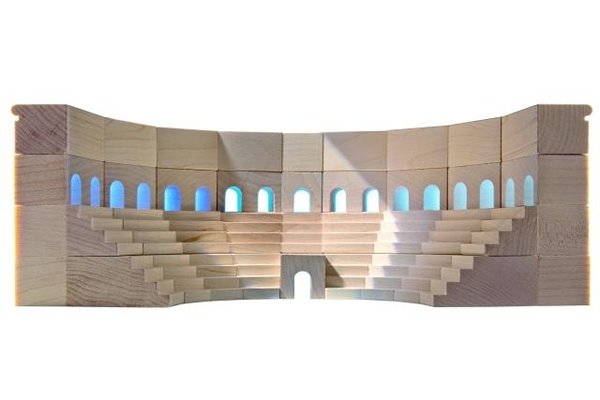
\includegraphics[height=16em]{building-blocks.jpg}
\end{columns}
\end{frame}

\begin{frame}
  \frametitle{Tools}

  \center{Replication is all about \textbf{tools}, not goals.}

\begin{columns}[c]
\column{.5\textwidth} 

  \begin{itemize}
    \item Hot Standby
    \item Streaming Replication
    \item Cascading Replication
    \item Skytools: londiste, PGQ
  \end{itemize}  

\column{.5\textwidth}
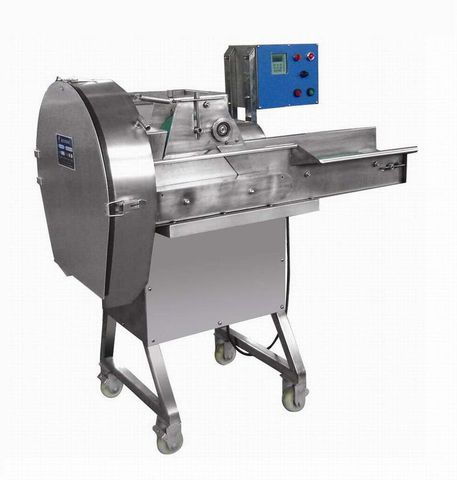
\includegraphics[height=15em]{multi_function_equipment.jpg}
\end{columns}
\end{frame}

\begin{frame}
  \frametitle{Architectures Examples}

\begin{columns}[c]
\column{.25\textwidth} 
\column{.75\textwidth} 
  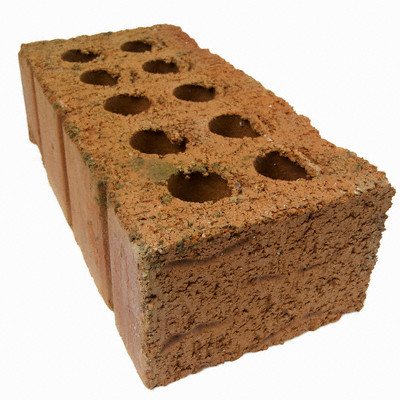
\includegraphics[height=16em]{brick-large.jpg}
\end{columns}
\end{frame}

\begin{frame}
  \frametitle{Load balancing reads: streaming replication}

  \includegraphics[height=16em]{archi_lb.png}
\end{frame}

\begin{frame}
  \frametitle{PGQ: efficient queueing in PostgreSQL}

\begin{columns}[c]
\column{.1\textwidth} 
\column{.9\textwidth} 
  
\includegraphics[height=16em]{coop-workers.jpeg}
\end{columns}
\end{frame}

\begin{frame}
  \frametitle{Load balancing writes: plproxy}

  \includegraphics[height=16em]{archi_plproxy.png}
\end{frame}

\begin{frame}
  \frametitle{Multiple Active Nodes: federation}

\begin{columns}[c]
\column{.25\textwidth} 
\column{.75\textwidth} 
  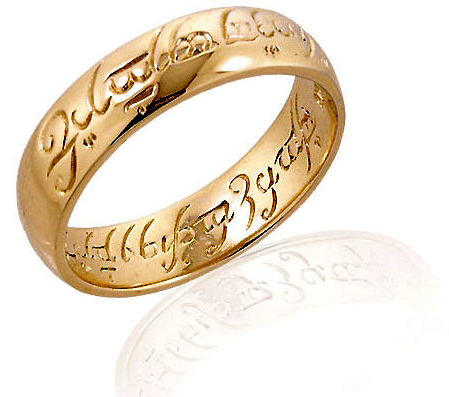
\includegraphics[height=16em]{the-one-ring.jpg}
\end{columns}
\end{frame}

\begin{frame}
  \frametitle{Multiple Active Nodes: federation}

  \includegraphics[height=14em]{archi_federated.png}
\end{frame}

\begin{frame}
  \frametitle{Multiple Active Nodes: split responsibility}

\begin{columns}[c]
\column{.1\textwidth} 
\column{.9\textwidth} 
  
\includegraphics[height=16em]{clock-key.jpg}
\end{columns}
\end{frame}

\begin{frame}
  \frametitle{Multiple Active Nodes: split responsibility}

  \includegraphics[height=14em]{archi_split.png}
\end{frame}

\section{Conclusion}

\frame{
  \frametitle{Questions?}

\begin{center}
  Now is the time to ask!
  \vfill

  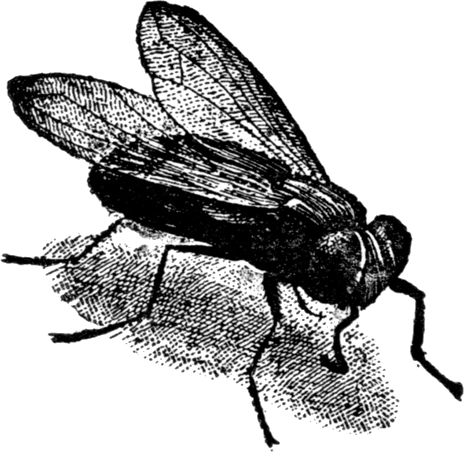
\includegraphics[height=9em]{fly.png}
\end{center}
}
\end{document}
